\appendix
%\include{chapter-appendix}

\begingroup
\clearpage% Manually insert \clearpage
\let\clearpage\relax% Remove \clearpage functionality
\vspace*{-16pt}% Insert needed vertical retraction
\chapter*{\centerline{APPENDICES}}
\endgroup

% \begin{center}
% {\bfseries Title of Appendix (Not Numbered)}
% \end{center}

\section*{Title of Appendix (Not Numbered)}
\addcontentsline{toc}{chapter}{APPENDICES}
\renewcommand{\thechapter}{A}
\numberwithin{equation}{chapter}
\setcounter{equation}{0}
%\setcounter{theorem}{0}

\subsection{Upgraded Tracking System} % MOVE TO HL-LHC Introduction section or PILEUP section

For the High-Luminosity LHC (HL-LHC), the ATLAS inner detector will be replaced entirely by the all-silicon Inner Tracker (ITk)~\cite{}. The HL-LHC will deliver instantaneous luminosities of up to $7 \times 10^{34}$\,cm$^{-2}$s$^{-1}$\cite{2105.10367}, resulting in an average of $\langle\mu\rangle \approx 200$ simultaneous $pp$ interactions per bunch crossing  (pile-up). The integrated luminosity is expected to reach 4000 $fb^{-1}$ by the end of the HL-LHC program, a significant increase from around 350 $fb^{-1}$ obtained in Run 3. As the current inner detector is inadequate for this radiation environment and track density, the TRT and SCT are fully decommissioned and replaced by the upgraded ITk. The ITk extends the tracking acceptance to $|\eta| < 4.0$, as illustrated in Figure~\ref{fig:ATLAS_ITk}, significantly improving forward track reconstruction for physics processes with boosted topologies and forward jets.

Strips: https://cds.cern.ch/record/2257755 \\
Upgrade Pixels: https://arxiv.org/abs/2105.10367

\begin{figure}[h]
	\centering
	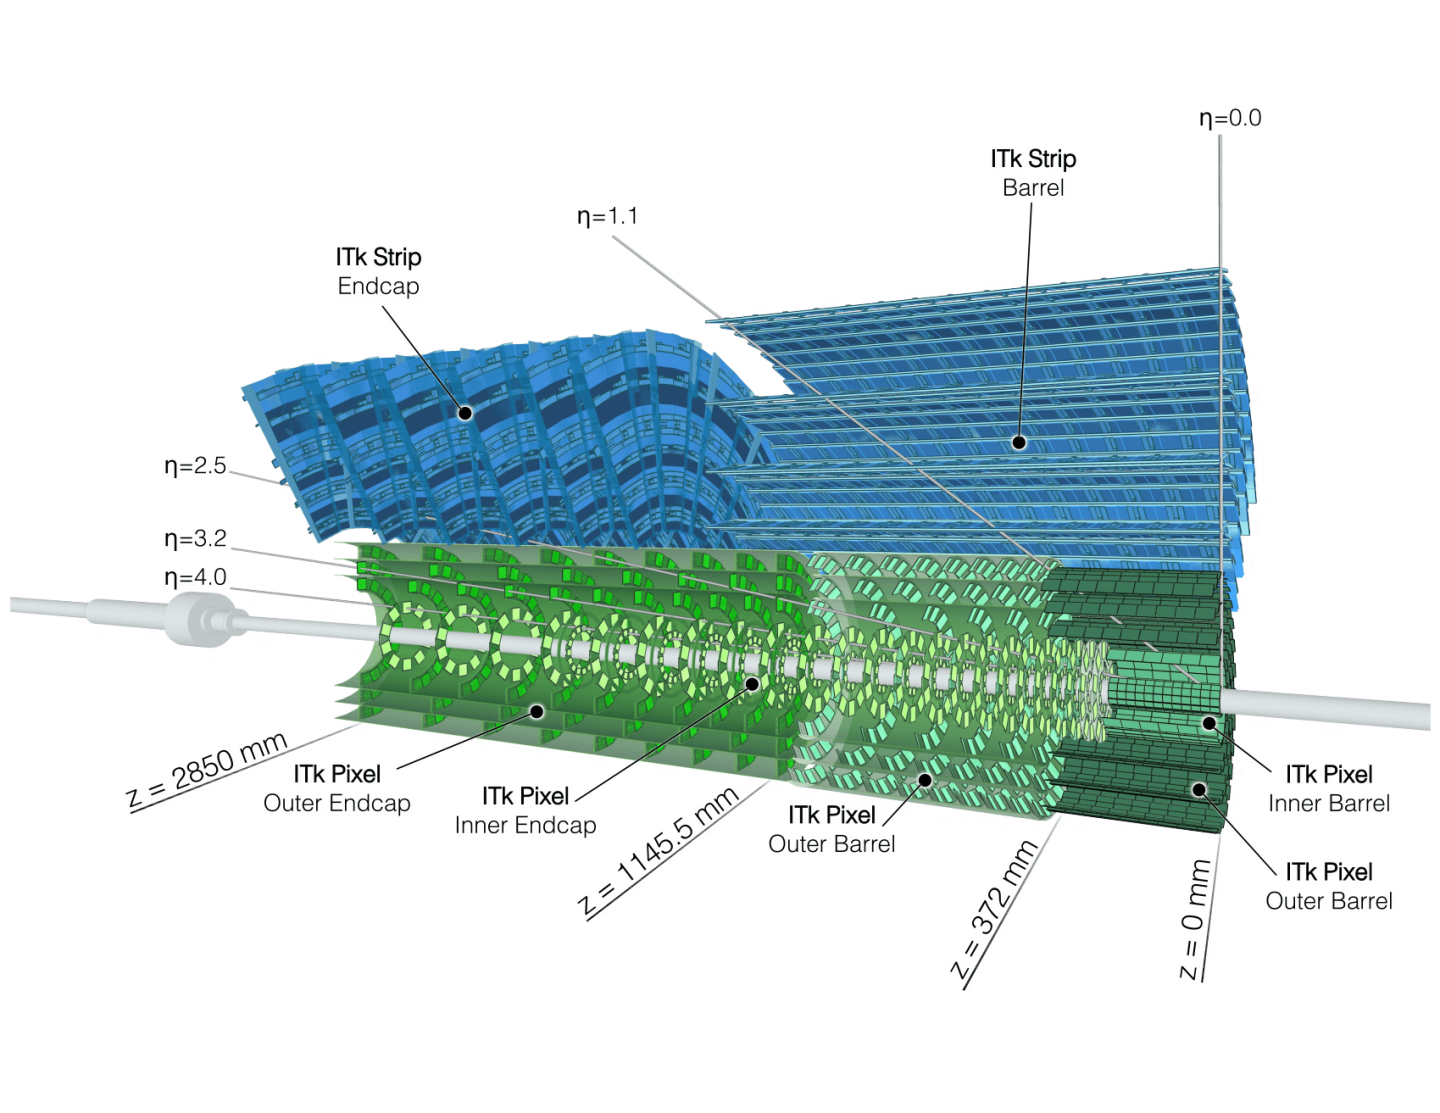
\includegraphics[width=0.7\linewidth]{figures/chapter3/ATLAS_tracker.png}
	\caption{https://atlas.cern/Resources/Schematics}
	\label{fig:ATLAS_ITk}
\end{figure}

The ITk comprises two subsystems. The ITk Pixel detector forms the innermost region, consisting of five barrel layers and multiple end-cap rings extending to $|z| = 2850$mm, as shown in Figure~\ref{fig:ATLAS_tracker}. With 5 billion readout channels, it provides high-granularity space-point measurements close to the interaction point, retaining excellent vertex resolution in the high pile-up environment. The ITk Strip detector surrounds the pixel system, consisting of four barrel layers extending to $|\eta| < 2.5$ and six end-cap discs on each side covering $1.1 < |\eta| < 4.0$. The strip detectors have 50 million readout channels, and strip modules use short strips of 24.1mm and 48.2mm length in the barrel and end-cap, respectively.


\lipsum[1]
